% =================================================================
% Presentación de la defensa del TFG (informe final)
% Duración objetivo: 20 min como máximo (19 láminas, ~1 min cada una)
% Compilar desde la raíz:  pdflatex Presentacion_Defensa.tex  (2 pasadas)
% Tiempos sugeridos entre corchetes en el comentario de cada lámina.
% =================================================================
\documentclass[aspectratio=169,11pt]{beamer}

\usepackage[utf8]{inputenc}
\usepackage[T1]{fontenc}
\usepackage{lmodern}
\usepackage[spanish,es-nodecimaldot]{babel}
\usepackage{graphicx}
\graphicspath{{imagenes/}}
\usepackage{booktabs}
\usepackage{tabularx}
\usepackage{array}
\usepackage{tikz}
\usetikzlibrary{positioning,arrows.meta,babel}
\usepackage{xcolor}

% -------------------------------------------------
% Colores (misma paleta del informe)
% -------------------------------------------------
\definecolor{DeepBlue}{HTML}{16324F}
\definecolor{ArduinoTeal}{HTML}{008184}
\definecolor{SoftBlue}{HTML}{EAF2FB}
\definecolor{TableGray}{HTML}{E9EBED}

\setbeamercolor{structure}{fg=DeepBlue}
\setbeamercolor{frametitle}{fg=white,bg=DeepBlue}
\setbeamercolor{title}{fg=DeepBlue}
\setbeamercolor{itemize item}{fg=ArduinoTeal}
\setbeamercolor{itemize subitem}{fg=ArduinoTeal}
\setbeamercolor{enumerate item}{fg=ArduinoTeal}
\setbeamercolor{block title}{fg=white,bg=ArduinoTeal}
\setbeamercolor{block body}{fg=black,bg=SoftBlue}
\setbeamercolor{footline}{fg=DeepBlue}

\setbeamertemplate{navigation symbols}{}
\setbeamertemplate{itemize items}[circle]
\setbeamerfont{frametitle}{size=\Large}
\setbeamerfont{block title}{size=\small}
\setbeamerfont{block body}{size=\small}
\setbeamerfont{itemize/enumerate body}{size=\small}
\setbeamerfont{itemize/enumerate subbody}{size=\footnotesize}

% Título de lámina en barra de color a todo el ancho
\setbeamertemplate{frametitle}{%
    \nointerlineskip
    \vskip-\headheight
    \begin{beamercolorbox}[wd=\paperwidth,ht=3.2ex,dp=1.4ex,leftskip=0.8cm]{frametitle}
        \usebeamerfont{frametitle}\insertframetitle
    \end{beamercolorbox}}

% Pie de lámina: autora y número
\setbeamertemplate{footline}{%
    \begin{beamercolorbox}[wd=\paperwidth,ht=2.6ex,dp=1.1ex,leftskip=0.8cm,rightskip=0.8cm]{footlinebar}
        {\scriptsize Plataforma didáctica para la enseñanza de PLC}%
        \hfill{\scriptsize\insertframenumber}
    \end{beamercolorbox}}
\setbeamercolor{footlinebar}{fg=white,bg=ArduinoTeal}

% Tablas: filas de encabezado en gris
\newcommand{\encabezado}{\rowcolor{TableGray}}
\usepackage{colortbl}

% Imagen con referencia al pie (como en Ejemplo_BEAMER): texto pequeño con la
% descripción y el número de referencia del informe, o "Fuente: Autora."
%   \figcap[opciones]{archivo}{pie}
\newcommand{\figcap}[3][]{\begin{tabular}[t]{@{}c@{}}\includegraphics[#1]{#2}\\[1pt]{\fontsize{6.5}{7.5}\selectfont #3}\end{tabular}}

% -------------------------------------------------
% Datos de portada
% -------------------------------------------------
\title[Plataforma didáctica para PLC]{Diseño de una plataforma didáctica para la enseñanza de PLC de la Escuela de Ingeniería Electrónica del Campus Tecnológico Local San Carlos}
\author{María del Milagro Rojas Sánchez}
\institute{Escuela de Ingeniería Electrónica\\Campus Tecnológico Local San Carlos\\[4pt]
\textbf{Asesor:} Ing. Pablo César Rodríguez Vargas}
\date{Noviembre 2026}

% =================================================================
\begin{document}
% =================================================================

% -------------------------------------------------
% 1. Portada [0:30]
% -------------------------------------------------
% Fondo azul como en Ejemplo_BEAMER; el logo es una copia con fondo
% transparente (imagenes/Logo_TEC_transparente.png) para que no se vea recuadro.
{
\setbeamercolor{background canvas}{bg=DeepBlue}
\begin{frame}[plain]
    \begin{tikzpicture}[remember picture,overlay]
        % franja inferior con los datos de autoría
        \fill[ArduinoTeal] (current page.south west) rectangle ([yshift=0.55cm]current page.south east);
        % logo en la esquina superior derecha
        \node[anchor=north east,inner sep=0] at ([xshift=-0.8cm,yshift=-0.5cm]current page.north east)
            {
\includegraphics[height=1.3cm]{Logo_TEC_transparente.png}};
        % título
        \node[anchor=west,text width=0.86\paperwidth,align=left,text=white,inner sep=0]
            at ([xshift=0.8cm,yshift=0.5cm]current page.west)
            {\hyphenpenalty=10000 {\LARGE Diseño de una plataforma didáctica para la enseñanza de PLC de la Escuela de Ingeniería Electrónica del Campus Tecnológico Local San Carlos\par}
             \vspace{0.35cm}
             {\normalsize Proyecto de graduación para optar por el grado de Licenciatura en Ingeniería Electrónica\par}};
        % autoría dentro de la franja
        \node[anchor=west,text=white,align=left,inner sep=0,font=\small]
            at ([xshift=0.8cm,yshift=1.55cm]current page.south west)
            {Autora: María del Milagro Rojas Sánchez\\[3pt]
             Asesor: Ing. Pablo César Rodríguez Vargas};
        \node[anchor=east,text=white,inner sep=0,font=\small]
            at ([xshift=-0.8cm,yshift=1.2cm]current page.south east)
            {Noviembre de 2026};
    \end{tikzpicture}
\end{frame}
}

% -------------------------------------------------
% Lámina de enganche (foto con velo oscuro, como en el ejemplo)
% -------------------------------------------------
{
\setbeamercolor{background canvas}{bg=black}
\setbeamertemplate{background}{%
    \begin{tikzpicture}[remember picture,overlay]
        \node[inner sep=0] at (current page.center){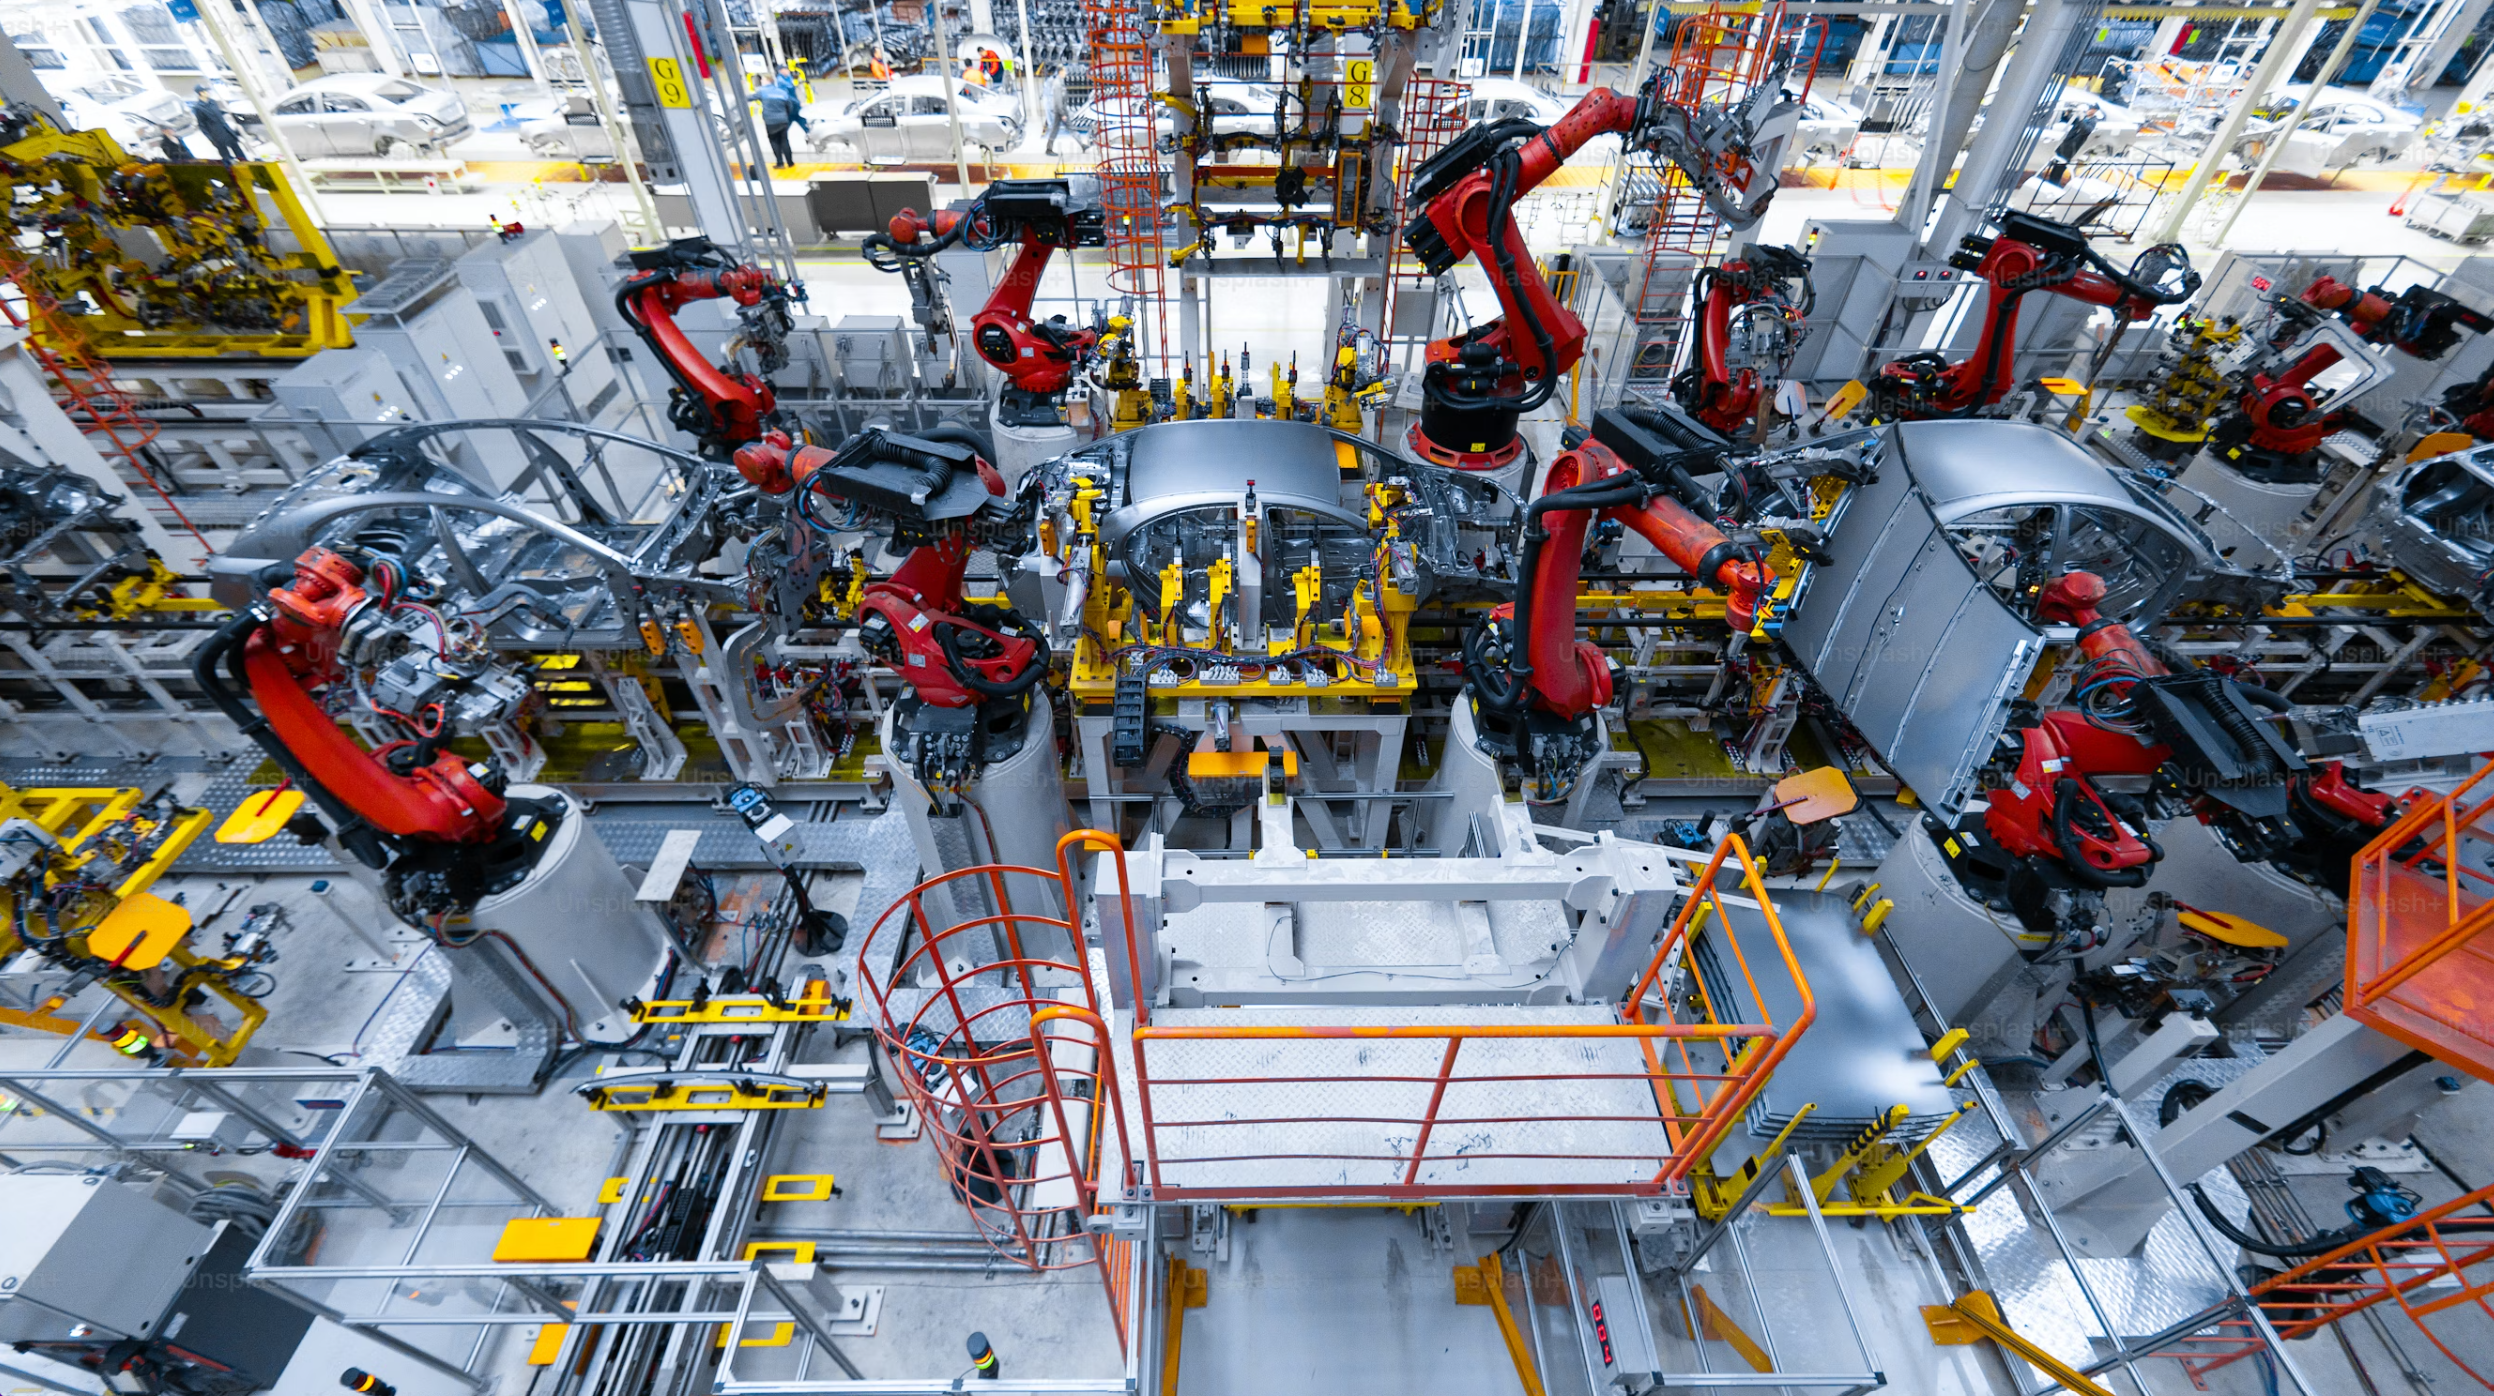
\includegraphics[width=\paperwidth,height=\paperheight]{Vista aerea de fabrica de automoviles.png}};
        \fill[black,opacity=0.7] (current page.south west) rectangle (current page.north east);
    \end{tikzpicture}}
\begin{frame}[plain]
    \vfill
    \centering{\color{white}\Large ¿Cómo se le enseña al futuro ingeniero\\lo que la industria ya exige hoy?\par}
    \vfill
    \begin{tikzpicture}[remember picture,overlay]
        \node[anchor=south west,inner sep=0,text=white,font=\fontsize{6.5}{7.5}\selectfont]
            at ([xshift=0.3cm,yshift=0.2cm]current page.south west) {Fuente: Unsplash [9]};
    \end{tikzpicture}
\end{frame}
}

% -------------------------------------------------
% 2. Contenido [0:30]
% -------------------------------------------------
\begin{frame}{Agenda}
    \begin{itemize}
        \setlength{\itemsep}{0.35em}
        \item Problema, meta y objetivos
        \item Procedimiento metodológico
        \item Descripción de la solución
        \item Resultados y análisis
        \item Costo-beneficio
        \item Conclusiones y recomendaciones
    \end{itemize}
\end{frame}

% -------------------------------------------------
% 3. Problema [1:30]
% -------------------------------------------------
\begin{frame}{El problema}
    \begin{columns}[T]
        \column{0.97\textwidth}
        \begin{itemize}
            \item El programa no cuenta con equipamiento dedicado a la enseñanza de automatización con PLC.
            \item Las competencias a 24~V~DC con IEC~61131-3 requieren hardware real, no solo simulación.
            \item Los equipos industriales y kits comerciales son costosos y cerrados: cambiar de práctica exige recablear.
            \item Automatización (24~V) y electrónica del estudiante (5~V) quedan desconectadas sin aislamiento.
        \end{itemize}
    \end{columns}
    \vspace{0.3cm}
    \begin{block}{Síntesis}
        Falta un entorno de experimentación para desarrollar competencias prácticas de forma segura, rigurosa y escalable.
    \end{block}
\end{frame}

% -------------------------------------------------
% 4. Meta y objetivos [1:30]
% -------------------------------------------------
\begin{frame}{Meta y objetivos}
    \begin{block}{Meta}
        Que estudiantes y docentes del Campus cuenten con un recurso experimental funcional para la enseñanza de automatización industrial con PLC.
    \end{block}
    \begin{block}{Objetivo general}
        Diseñar una plataforma didáctica modular para la enseñanza de PLC, con tecnología Arduino Opta e instrumentación de bajo costo, que garantice la integridad eléctrica del sistema.
    \end{block}
    \textbf{Objetivos específicos}
    \begin{enumerate}
        \item Diseñar el panel de control con el PLC y sus módulos, y terminales accesibles para conectar dispositivos de campo a 24~V~DC.
        \item Verificar el funcionamiento con experimentos de adquisición de señales y lógica de control programada.
        \item Comparar el costo-beneficio frente a PLC industriales convencionales.
    \end{enumerate}
\end{frame}

% -------------------------------------------------
% 5. Base tecnológica [1:00]
% -------------------------------------------------
\begin{frame}{Base tecnológica: Arduino PLC Starter Kit}
    \begin{columns}[T]
        \column{0.5\textwidth}
        \centering
        \figcap[width=0.95\linewidth]{PLC_Starter_Kit_Arduino_Store.jpg}{Arduino PLC Starter Kit (AKX00051) [2]}
        \column{0.5\textwidth}
        \begin{itemize}
            \item Arduino Opta WiFi: controlador con 8 entradas de 0 a 24~V~DC y 4 salidas de relé; Ethernet, WiFi, USB-C y RS-485.
            \item DIN Simul8 (interruptores) y DIN Celsius (sensor y calentadores).
            \item Expansión AFX00007 (A0602): entradas analógicas (0--10~V, 4--20~mA, RTD), salidas analógicas y PWM.
            \item Programación en Arduino PLC IDE, gratuito, con lenguajes IEC~61131-3.
        \end{itemize}
    \end{columns}
\end{frame}

% -------------------------------------------------
% 6. Metodología [1:00]
% -------------------------------------------------
\begin{frame}{Procedimiento metodológico}
    \begin{center}
    \figcap[width=0.9\linewidth,height=0.3\textheight,keepaspectratio,trim=29 42 66 41,clip]{Diagrama_Metodologia.pdf}{Procedimiento metodológico (draw.io). Fuente: Autora.}
    \end{center}
    \vspace{0.3cm}
    \begin{itemize}
        \item Cada decisión de diseño se tomó con una matriz de Pugh: criterios con peso (suma 1,00), puntajes de 1 a 5 y puntaje ponderado.
        \item Se evaluaron tres decisiones de arquitectura: unidad de control, material estructural e interfaz de acoplamiento.
    \end{itemize}
\end{frame}

% -------------------------------------------------
% 7. Selección de unidad de control [1:00]
% -------------------------------------------------
\begin{frame}{Selección de la unidad de control}
    \begin{columns}[T]
        \column{0.5\textwidth}
        \renewcommand{\arraystretch}{1.25}
        \begin{tabular}{|l|c|}
            \hline
            \encabezado \textbf{Alternativa} & \textbf{Puntaje (1--5)} \\ \hline
            Arduino Opta & 4,62 \\ \hline
            Siemens S7-1500 & 3,30 \\ \hline
            Festo EduTrainer & 3,23 \\ \hline
            Arduino UNO & 2,80 \\ \hline
            ESP32 & 2,74 \\ \hline
        \end{tabular}
        \vspace{0.3cm}

        \small Opta: PLC industrial real, entradas a 24~V, programación IEC~61131-3, bajo costo y entorno gratuito.
        \column{0.5\textwidth}
        \centering
        \figcap[height=2.1cm]{Arduino_OPTA_Estetico.png}{Arduino Opta WiFi [8]}\hfill
        \figcap[height=2.1cm]{PLC Siemens S7 1500.jpg}{Siemens S7-1500 [17]}\\[4pt]
        \figcap[height=1.6cm]{Edu_trainer.jpg}{Festo EduTrainer [18]}\hfill
        \figcap[height=1.6cm]{Arduino_UNO_R3.png}{Arduino UNO R3 [19]}\hfill
        \figcap[height=1.6cm]{esp32.png}{ESP32 [20]}
    \end{columns}
\end{frame}

% -------------------------------------------------
% 8. Otras selecciones [1:00]
% -------------------------------------------------
\begin{frame}{Selección de estructura e interfaz de acoplamiento}
    \begin{columns}[T]
        \column{0.5\textwidth}
        \centering\small\textbf{Material estructural}\\[3pt]
        \renewcommand{\arraystretch}{1.2}
        \begin{tabular}{@{}c@{\hspace{0.3cm}}c@{}}
        \begin{tabular}{|l|c|}
            \hline
            Perfil T-slot & 4,70 \\ \hline
            Madera & 3,26 \\ \hline
            Impresión 3D & 2,97 \\ \hline
            PVC & 2,56 \\ \hline
            Acero & 2,48 \\ \hline
        \end{tabular} &
        \figcap[height=1.8cm]{T-Slot_20x20.jpg}{Perfil T-slot 20x20 [*]}
        \end{tabular}
        \begin{itemize}\small
            \item Modular: se arma sin soldadura.
            \item Uniones atornilladas: piezas fáciles de cambiar.
        \end{itemize}
        \column{0.5\textwidth}
        \centering\small\textbf{Interfaz de acoplamiento}\\[3pt]
        \renewcommand{\arraystretch}{1.2}
        \begin{tabular}{@{}c@{\hspace{0.3cm}}c@{}}
        \begin{tabular}{|l|c|}
            \hline
            Optoacoplador PC817 & 4,88 \\ \hline
            4N25 & 2,80 \\ \hline
            Módulo MOSFET & 2,66 \\ \hline
        \end{tabular} &
        \figcap[width=3.2cm,height=1.8cm,keepaspectratio]{Optoacoplador_PC817.png}{Tarjeta PC817 [13]}
        \end{tabular}
        \begin{itemize}\small
            \item Ya viene montada en placa, con bornes atornillables.
            \item Cuatro canales aislables (4N25 y MOSFET, uno).
        \end{itemize}
    \end{columns}
\end{frame}

% -------------------------------------------------
% 9. Estructura de soporte [1:00]
% -------------------------------------------------
\begin{frame}{Estructura de soporte}
    \begin{columns}[T]
        \column{0.5\textwidth}
        \centering
        \figcap[width=0.85\linewidth,height=0.62\textheight,keepaspectratio]{Producto_estructura_esperado.png}{Modelo de ensamble de la estructura de soporte. Fuente: Autora.}
        \column{0.5\textwidth}
        \begin{itemize}
            \item Criterios de diseño: mínimo material, resistencia y confort del estudiante.
            \item Aluminio T-slot: plan de corte de seis perfiles.
            \item Panel de acrílico inclinado 70° para facilitar la visibilidad y el acceso a las borneras.
            \item Piezas de unión impresas en 3D (ángulo delantero y codo trasero) que fijan los 70°.
        \end{itemize}
        \centering
        \figcap[height=1.3cm]{Pieza_delantera_angulo_vistalateral.png}{Pieza delantera. Fuente: Autora.}\hspace{0.3cm}
        \figcap[height=1.3cm]{Pieza_trasera_codo_vistaperfil.png}{Codo trasero. Fuente: Autora.}
    \end{columns}
\end{frame}

% -------------------------------------------------
% 10. Plataforma completa [1:15]
% -------------------------------------------------
\begin{frame}{La plataforma terminada}
    \begin{columns}[T]
        \column{0.35\textwidth}
        \centering
        \figcap[height=0.68\textheight]{Plataforma_completa.jpeg}{Plataforma terminada. Fuente: Autora.}
        \column{0.65\textwidth}
        \begin{itemize}
            \item Riel 1: Arduino Opta WiFi y expansión analógica A0602.
            \item Riel 2: borneras de alimentación X24V y X0V, tarjeta optoacopladora PC817 y Simul8.
            \item Riel 3: borneras etiquetadas, donde el estudiante hace sus conexiones.
            \item Toda la plataforma queda a la vista; el estudiante trabaja sobre las borneras etiquetadas y no sobre los bornes del controlador.
            \item Alimentación única de 24~V~DC con el adaptador del kit.
        \end{itemize}
    \end{columns}
\end{frame}

% -------------------------------------------------
% 11. Regleta y código de colores [1:00]
% -------------------------------------------------
\begin{frame}{Borneras de conexión e identificación}
    \begin{columns}[T]
        \column{0.5\textwidth}
        \centering
        \figcap[height=0.72\textheight]{panel_hecho_drawio.png}{Distribución del panel de control (draw.io). Fuente: Autora.}
        \column{0.5\textwidth}
        \begin{itemize}
            \item Ocho grupos rotulados que siguen la secuencia de entradas y salidas: EasyPort, optoacoplador, entradas digitales, salidas de relé, entradas analógicas, salida analógica, PWM y 24~V.
            \item Código de colores por tipo de señal.
            \item Etiqueta numérica por canal; rojo~1 = +24~V y negro~0 = GND.
            \item Alimentación separada de las señales.
            \item Continuidad verificada en todas las conexiones.
        \end{itemize}
    \end{columns}
\end{frame}

% -------------------------------------------------
% 12. Diagrama eléctrico [0:45]
% -------------------------------------------------
\begin{frame}{Diagrama eléctrico de la plataforma}
    \centering
    \figcap[width=0.95\linewidth,height=0.72\textheight,keepaspectratio]{Diagrama_Electrico_Plataforma.pdf}{Diagrama eléctrico de la plataforma. Fuente: Autora.}
\end{frame}

% -------------------------------------------------
% 13. Interfaz de aislamiento [1:00]
% -------------------------------------------------
\begin{frame}{Interfaz de aislamiento para circuitos de baja tensión}
    \begin{columns}[T]
        \column{0.45\textwidth}
        \centering
        \figcap[width=0.9\linewidth]{Optoacoplador_PC817.png}{Tarjeta optoacopladora de cuatro canales basada en el PC817 [13]}
        \column{0.55\textwidth}
        \begin{itemize}
            \item Tarjeta optoacopladora PC817 de cuatro canales aislados.
            \item Las salidas del PLC (24~V) gobiernan circuitos propios del estudiante, alimentados con su propia fuente de 3,6 a 30~V (habitualmente 5~V).
            \item Sin contacto eléctrico entre el lado industrial y el lado electrónico.
            \item Une la automatización a 24~V con lo que el estudiante construye en los demás laboratorios.
        \end{itemize}
    \end{columns}
\end{frame}

% -------------------------------------------------
% 14. Práctica 1 [1:30]
% -------------------------------------------------
\begin{frame}{Práctica 1: secuencia de cinco estados}
    \begin{columns}[T]
        \column{0.45\textwidth}
        \begin{itemize}
            \item Proceso secuencial de una línea de producción: cuatro actuadores activados uno tras otro, con pulsadores de arranque y parada.
            \item Programa en Ladder Diagram; planta neumática simulada en FluidSIM.
            \item El Opta se enlaza con FluidSIM por el EasyPort USB.
            \item Valida: entradas digitales, salidas de relé y la capacidad del controlador para gobernar una planta virtual.
        \end{itemize}
        \column{0.55\textwidth}
        \centering
        \figcap[width=\linewidth,height=0.66\textheight,keepaspectratio,trim=6 290 0 8,clip]{Diagrama_Electrico_Practica1.pdf}{Conexiones usadas en la Práctica 1. Fuente: Autora.}
    \end{columns}
\end{frame}

% -------------------------------------------------
% 15. Práctica 2 [2:00]
% -------------------------------------------------
\begin{frame}{Práctica 2: enfriamiento con ventilación regulable}
    \begin{columns}[T]
        \column{0.5\textwidth}
        \begin{itemize}
            \item Sistema de enfriamiento: DIN Celsius = recinto; calentadores = cargas térmicas; motor de 24~V = ventilador.
            \item Programa en Ladder Diagram con control proporcional y referencia de 28~$^\circ$C.
            \item Salida por PWM y por salida analógica de 0 a 10~V (EasyPort).
            \item Resultado: al encender los calentadores con pulsadores, la temperatura aumenta y el controlador incrementa las salidas PWM y analógica.
            \item Valida: entradas digitales, entrada analógica, PWM y salida analógica.
        \end{itemize}
        \column{0.5\textwidth}
        \centering
        \figcap[width=\linewidth,height=0.66\textheight,keepaspectratio,trim=6 290 0 8,clip]{Diagrama_Electrico_Practica2.pdf}{Conexiones usadas en la Práctica 2. Fuente: Autora.}
    \end{columns}
\end{frame}

% -------------------------------------------------
% 16. Cobertura de señales [1:00]
% -------------------------------------------------
\begin{frame}{Análisis: señales verificadas}
    \footnotesize
    \renewcommand{\arraystretch}{1.35}
    \begin{tabular}{|p{3.3cm}|p{6.6cm}|c|}
        \hline
        \encabezado \textbf{Tipo de señal} & \textbf{Dispositivo de prueba} & \textbf{Práctica} \\ \hline
        Entrada digital de 24~V & Pulsadores e interruptores del DIN Simul8 & 1 y 2 \\ \hline
        Salida de relé & Entradas del EasyPort (FluidSIM); calentadores del DIN Celsius & 1 y 2 \\ \hline
        Entrada analógica 0--10~V & Sensor TMP236 del DIN Celsius & 2 \\ \hline
        Salida PWM & Motor de corriente continua de 24~V & 2 \\ \hline
        Salida analógica 0--10~V & Multímetro y entrada analógica del EasyPort & 2 \\ \hline
    \end{tabular}
    \normalsize
    \vspace{0.3cm}
    \begin{itemize}
        \item Entre las dos prácticas quedaron validados los cinco tipos de señal de la plataforma.    \end{itemize}
\end{frame}

% -------------------------------------------------
% 17. Costo-beneficio [1:30]
% -------------------------------------------------
\begin{frame}{Costo-beneficio frente a PLC industriales}
    \begin{columns}[T]
        \column{0.62\textwidth}
        \centering
        \begin{tikzpicture}[x=1cm,y=1cm,
            barra/.style={minimum height=0.7cm,anchor=west,inner sep=0pt}]
            % escala: 1,6 cm = 1 millón de colones (valores en millones)
            \def\esc{1.3}
            \node[anchor=east,font=\scriptsize,align=right] at (0,2.4) {Plataforma\\(presupuesto total)};
            \fill[ArduinoTeal] (0,2.05) rectangle (0.478780*\esc,2.75);
            \node[anchor=west,font=\scriptsize] at (0.478780*\esc+0.1,2.4) {₡478\,780};

            \node[anchor=east,font=\scriptsize,align=right] at (0,1.2) {S7-1500\\(hardware)};
            \fill[DeepBlue!60] (0,0.85) rectangle (1.259712*\esc,1.55);
            \node[anchor=west,font=\scriptsize] at (1.259712*\esc+0.1,1.2) {₡1\,259\,712};

            \node[anchor=east,font=\scriptsize,align=right] at (0,0) {S7-1500\\(con licencia)};
            \fill[DeepBlue] (0,-0.35) rectangle (3.279853*\esc,0.35);
            \node[anchor=west,font=\scriptsize] at (3.279853*\esc+0.1,0) {₡3\,279\,853};

            \node[anchor=east,font=\scriptsize,align=right] at (0,-1.2) {EduTrainer\\(equipo base)};
            \fill[DeepBlue!80!black] (0,-1.55) rectangle (3.856707*\esc,-0.85);
            \node[anchor=west,font=\scriptsize] at (3.856707*\esc+0.1,-1.2) {₡3\,856\,707};
        \end{tikzpicture}
        \column{0.38\textwidth}
        \begin{itemize}
            \item S7-1500: 2,6$\times$ el presupuesto en hardware y 6,9$\times$ con licencia STEP~7.
            \item EduTrainer: 8,1$\times$ el presupuesto de la plataforma.
            \item Como el S7-1500 y el EduTrainer, la plataforma ofrece lo esencial para enseñar PLC: IEC~61131-3, 24~V, comunicación y ampliación modular.
            \item Con la ventaja de un entorno de programación gratuito.
        \end{itemize}
    \end{columns}
\end{frame}

% -------------------------------------------------
% 18. Conclusiones [1:30]
% -------------------------------------------------
\begin{frame}{Conclusiones}
    \begin{itemize}
        \item Se diseñó y montó una plataforma modular con Arduino Opta que ejecuta prácticas completas de PLC con IEC~61131-3 y señales a 24~V~DC (objetivo general).
        \item El panel concentra las conexiones en ocho grupos de borneras rotuladas, con código de colores y alimentación separada (objetivo específico~1).
        \item Dos prácticas en Ladder validaron los cinco tipos de señal con dispositivos de bajo costo, y la guía de laboratorio las documenta (objetivo específico~2).
        \item Un puesto convencional cuesta 2,6 a 8,1 veces más, con funcionalidad comparable para la docencia (objetivo específico~3).
        \item La plataforma se integra con equipos y entornos virtuales (EasyPort, FluidSIM) y su tarjeta PC817 une el mundo de 24~V con la electrónica del estudiante.
        \item Plataforma y guía quedan listas para incorporarse a los cursos de la carrera.
    \end{itemize}
\end{frame}

% -------------------------------------------------
% 19. Recomendaciones y cierre [1:00]
% -------------------------------------------------
\begin{frame}{Recomendaciones y trabajo futuro}
    \begin{columns}[T]
        \column{0.55\textwidth}
        \textbf{Para reproducir la plataforma}
        \begin{itemize}
            \item Cotizar de nuevo los componentes antes de cada réplica.
            \item Imprimir las piezas de unión en ABS.
            \item Retirar los puentes de tierra de la PC817.
            \item Mantener una alimentación general única, para conservar la misma referencia de tensión en toda la plataforma.
            \item Usar sensores de tipo PNP, que se conectan directamente a las entradas del Opta.
        \end{itemize}
        \column{0.45\textwidth}
        \textbf{Para ampliar su uso}
        \begin{itemize}
            \item Evaluar el efecto en el aprendizaje al usarla en los cursos.
            \item Agregar más expansiones, analógicas y digitales, sin superar el límite de cinco por controlador.
            \item Cablear la comunicación Modbus, documentada en este proyecto.
        \end{itemize}
    \end{columns}
\end{frame}

% -------------------------------------------------
% Referencias de las imágenes (numeración del informe)
% -------------------------------------------------
\begin{frame}{Referencias (1/2)}
    \scriptsize
    \begin{description}\setlength{\itemsep}{1pt}
        \item[{[1]}] Arduino, ``Opta: Hardware Documentation,'' \emph{Arduino Documentation}.
        \item[{[2]}] Arduino Education, ``PLC Starter Kit,'' \emph{Arduino}.
        \item[{[8]}] Arduino, ``Opta User Manual,'' \emph{Arduino Documentation}.
        \item[{[9]}] Unsplash, ``Producción en línea de montaje de automóviles: brazo robótico en línea de producción,'' \emph{Unsplash}.
        \item[{[13]}] CRCibernética, ``PC817 Optocoupler Board,'' \emph{CRCibernética}.
        \item[{[14]}] Sharp Corporation, ``PC817 Series: High Density Mounting Type Photocoupler,'' hoja de datos.
        \item[{[15]}] CRCibernética, ``Optocoupler MOSFET Driver Module,'' \emph{CRCibernética}.
        \item[{[16]}] CRCibernética, ``4N25 DIP-6 Optocoupler,'' \emph{CRCibernética}.
        \item[{[17]}] Relepro, ``Siemens SIMATIC S7-1500 CPU 1513-1 PN (6ES7513-1AL02-0AB0),'' \emph{Relepro}.
        \item[{[18]}] Festo, ``Opciones preferidas de EduTrainer Universal para laboratorio con SIMATIC S7-1500.''
        \item[{[19]}] MicroJPM, ``Arduino UNO R3 [versión genérica], AD20477,'' \emph{MicroJPM}.
        \item[{[20]}] MicroJPM, ``ESP-32 Development Board 2.4 GHz Dual-Mode WiFi + Bluetooth, AD42922,'' \emph{MicroJPM}.
    \end{description}
\end{frame}

% -------------------------------------------------
% Referencias (2/2)
% -------------------------------------------------
\begin{frame}{Referencias (2/2)}
    \scriptsize
    \begin{description}\setlength{\itemsep}{1pt}
        \item[{[27]}] Festo Didactic SE, \emph{EasyPort USB: Manual}, ref.~721876, 2011.
        \item[{[28]}] Festo, ``Simulation software FluidSIM,'' \emph{Festo}.
        \item[{[35]}] Arduino, ``Arduino Opta Analog Expansion: Product Reference Manual (AFX00007),'' hoja de datos.
        \item[{[36]}] Arduino, ``Arduino PLC Starter Kit: Product Reference Manual (AKX00051),'' hoja de datos.
        \item[{[37]}] Arduino, ``Arduino DIN Celsius: Product Reference Manual (ABX00098),'' hoja de datos.
        \item[{[38]}] International Electrotechnical Commission, \emph{IEC 61131-3: Programmable controllers. Part 3: Programming languages}, 2013.
        \item[{[42]}] Relepro, ``SIMATIC S7-1500, DI 16X24VDC HF (6ES7521-1BH00-0AB0),'' \emph{Relepro}.
        \item[{[43]}] Relepro, ``SIMATIC S7-1500, módulo de salidas digitales DQ 16x24VDC/0,5A (6ES7522-1BH01-0AB0),'' \emph{Relepro}.
        \item[{[44]}] Relepro, ``SIMATIC S7-1500, alimentación de sistema PS 25W 24 DC (6ES7505-0KA00-0AB0),'' \emph{Relepro}.
        \item[{[45]}] Relepro, ``SIMATIC S7-1500, perfil soporte 245 mm (6ES7590-1AC40-0AA0),'' \emph{Relepro}.
        \item[{[46]}] Lieske, ``Siemens SIMATIC STEP 7 Professional V19, licencia flotante, descarga (6ES7822-1AA23-0YA5),'' \emph{Industry-Electronics}.
        \item[{[47]}] ICE Electronics International S.A., ``Cotización N.º ICEE23102024A: PLC EduTrainer Universal Siemens,'' San José, Costa Rica, 23-oct-2024.
    \end{description}
\end{frame}

% -------------------------------------------------
% Lámina final de agradecimiento (mismo estilo que la portada)
% -------------------------------------------------
{
\setbeamercolor{background canvas}{bg=DeepBlue}
\begin{frame}[plain]
    \begin{tikzpicture}[remember picture,overlay]
        \fill[ArduinoTeal] (current page.south west) rectangle ([yshift=0.55cm]current page.south east);
        \node[anchor=north east,inner sep=0] at ([xshift=-0.8cm,yshift=-0.5cm]current page.north east)
            {
\includegraphics[height=1.3cm]{Logo_TEC_transparente.png}};
        \node[text=white,align=center,inner sep=0] at (current page.center)
            {{\fontsize{30}{36}\selectfont Gracias por su atención\par}};
    \end{tikzpicture}
\end{frame}
}

\end{document}
